%package list
\documentclass{article}
\usepackage[top=3cm, bottom=3cm, outer=3cm, inner=3cm]{geometry}
\usepackage{multicol}
\usepackage{graphicx}
\usepackage{url}
%\usepackage{cite}
\usepackage{hyperref}
\usepackage{array}
%\usepackage{multicol}
\newcolumntype{x}[1]{>{\centering\arraybackslash\hspace{0pt}}p{#1}}
\usepackage{natbib}
\usepackage{pdfpages}
\usepackage{multirow}
\usepackage[normalem]{ulem}
\useunder{\uline}{\ul}{}
\usepackage{svg}
\usepackage{xcolor}
\usepackage{listings}
\lstdefinestyle{ascii-tree}{
    literate={├}{|}1 {─}{--}1 {└}{+}1 
  }
\lstset{basicstyle=\ttfamily,
  showstringspaces=false,
  commentstyle=\color{red},
  keywordstyle=\color{blue}
}
%\usepackage{booktabs}
\usepackage{caption}
\usepackage{subcaption}
\usepackage{float}
\usepackage{array}

\newcolumntype{M}[1]{>{\centering\arraybackslash}m{#1}}
\newcolumntype{N}{@{}m{0pt}@{}}


%%%%%%%%%%%%%%%%%%%%%%%%%%%%%%%%%%%%%%%%%%%%%%%%%%%%%%%%%%%%%%%%%%%%%%%%%%%%
%%%%%%%%%%%%%%%%%%%%%%%%%%%%%%%%%%%%%%%%%%%%%%%%%%%%%%%%%%%%%%%%%%%%%%%%%%%%
\newcommand{\itemEmail}{jquispemad@unsa.edu.pe}
\newcommand{\itemStudent}{JefersonJofre Quispe Madariaga}
\newcommand{\itemCourse}{Programación}
\newcommand{\itemCourseCode}{20232200}
\newcommand{\itemSemester}{II}
\newcommand{\itemUniversity}{Universidad Nacional de San Agustín de Arequipa}
\newcommand{\itemFaculty}{Facultad de Ingeniería de Producción y Servicios}
\newcommand{\itemDepartment}{Departamento Académico de Ingeniería de Sistemas e Informática}
\newcommand{\itemSchool}{Escuela Profesional de Ingeniería de Sistemas}
\newcommand{\itemAcademic}{2023 - B}
\newcommand{\itemInput}{Del 15 Enero 2024}
\newcommand{\itemOutput}{Al 22 Enero 2024}
\newcommand{\itemPracticeNumber}{22}
\newcommand{\itemTheme}{Interfaz Gráfica de Usuario}
%%%%%%%%%%%%%%%%%%%%%%%%%%%%%%%%%%%%%%%%%%%%%%%%%%%%%%%%%%%%%%%%%%%%%%%%%%%%
%%%%%%%%%%%%%%%%%%%%%%%%%%%%%%%%%%%%%%%%%%%%%%%%%%%%%%%%%%%%%%%%%%%%%%%%%%%%

\usepackage[english,spanish]{babel}
\usepackage[utf8]{inputenc}
\AtBeginDocument{\selectlanguage{spanish}}
\renewcommand{\figurename}{Figura}
\renewcommand{\refname}{Referencias}
\renewcommand{\tablename}{Tabla} %esto no funciona cuando se usa babel
\AtBeginDocument{%
	\renewcommand\tablename{Tabla}
}

\usepackage{fancyhdr}
\pagestyle{fancy}
\fancyhf{}
\setlength{\headheight}{30pt}
\renewcommand{\headrulewidth}{1pt}
\renewcommand{\footrulewidth}{1pt}
\fancyhead[L]{\raisebox{-0.2\height}{
\includegraphics[width=3cm]{img/logo_episunsa.png}}}
\fancyhead[C]{\fontsize{7}{7}\selectfont	\itemUniversity \\ \itemFaculty \\ \itemDepartment \\ \itemSchool \\ \textbf{\itemCourse}}
\fancyhead[R]{\raisebox{-0.2\height}{
\includegraphics[width=1.2cm]{img/logo_abet}}}
\fancyfoot[L]{Estud. Jeferson Jofre Quispe Madaraiaga}
\fancyfoot[C]{\itemCourse}
\fancyfoot[R]{Página \thepage}

% para el codigo fuente
\usepackage{listings}
\usepackage{color, colortbl}
\definecolor{dkgreen}{rgb}{0,0.6,0}
\definecolor{gray}{rgb}{0.5,0.5,0.5}
\definecolor{mauve}{rgb}{0.58,0,0.82}
\definecolor{codebackground}{rgb}{0.95, 0.95, 0.92}
\definecolor{tablebackground}{rgb}{0.8, 0, 0}

\lstset{frame=tb,
	language=bash,
	aboveskip=3mm,
	belowskip=3mm,
	showstringspaces=false,
	columns=flexible,
	basicstyle={\small\ttfamily},
	numbers=none,
	numberstyle=\tiny\color{gray},
	keywordstyle=\color{blue},
	commentstyle=\color{dkgreen},
	stringstyle=\color{mauve},
	breaklines=true,
	breakatwhitespace=true,
	tabsize=3,
	backgroundcolor= \color{codebackground},
}

\begin{document}
	
	\vspace*{10px}
	
	\begin{center}	
		\fontsize{17}{17} \textbf{ Informe de Laboratorio \itemPracticeNumber}
	\end{center}
	\centerline{\textbf{\Large Tema: \itemTheme}}
	%\vspace*{0.5cm}	

	\begin{flushright}
		\begin{tabular}{|M{2.5cm}|N|}
			\hline 
			\rowcolor{tablebackground}
			\color{white} \textbf{Nota}  \\
			\hline 
			     \\[30pt]
			\hline 			
		\end{tabular}
	\end{flushright}	

	\begin{table}[H]
		\begin{tabular}{|x{4.7cm}|x{4.8cm}|x{4.8cm}|}
			\hline 
			\rowcolor{tablebackground}
			\color{white} \textbf{Estudiante} & \color{white}\textbf{Escuela}  & \color{white}\textbf{Asignatura}   \\
			\hline 
			{\itemStudent \par \itemEmail} & \itemSchool & {\itemCourse \par Semestre: \itemSemester \par Código: \itemCourseCode}     \\
			\hline 			
		\end{tabular}
	\end{table}		
	
	\begin{table}[H]
		\begin{tabular}{|x{4.7cm}|x{4.8cm}|x{4.8cm}|}
			\hline 
			\rowcolor{tablebackground}
			\color{white}\textbf{Laboratorio} & \color{white}\textbf{Tema}  & \color{white}\textbf{Duración}   \\
			\hline 
			\itemPracticeNumber & \itemTheme & 04 horas   \\
			\hline 
		\end{tabular}
	\end{table}
	
	\begin{table}[H]
		\begin{tabular}{|x{4.7cm}|x{4.8cm}|x{4.8cm}|}
			\hline 
			\rowcolor{tablebackground}
			\color{white}\textbf{Semestre académico} & \color{white}\textbf{Fecha de inicio}  & \color{white}\textbf{Fecha de entrega}   \\
			\hline 
			\itemAcademic & \itemInput &  \itemOutput  \\
			\hline 
		\end{tabular}
	\end{table}
	
	\section{Tarea}
	\begin{itemize}		
		\item Interfaz Gráfica de Usuario
		\item Usar componentes básicos GUI: Etiquetas, botones, cuadros de texto, JOptionPane, Color.
		\item Usar componentes avanzados GUI: Layouts, JPanel, áreas de texto, checkbox, botones de radio y combobox.
	\end{itemize}
		
	\section{Equipos, materiales y temas utilizados}
	\begin{itemize}
		\item Sistema Operativo Ubuntu GNU Linux 23 lunar 64 bits Kernell 6.2.
		\item VIM 9.0.
		\item OpenJDK 64-Bits 17.0.7.
		\item Git 2.39.2.
		\item Cuenta en GitHub con el correo institucional.
		\item Programación Orientada a Objetos.
		\item Algoritmo de ordenamiento por inserción	
	\end{itemize}
	
	\section{URL de Repositorio Github}
	\begin{itemize}
		\item URL del Repositorio GitHub para clonar o recuperar.
		\item \url{https://github.com/jquispemad/fp2-23b.git}
		\item URL para el laboratorio 22 en el Repositorio GitHub.
		\item \url{https://github.com/jquispemad/fp2-23b/tree/main/fase_03/lab_22}
	\end{itemize}
	
	\section{Actividades con el repositorio GitHub}
	
	\subsection{Commits de lab 22}
\begin{itemize}		
		\item Mediante las importaciones con swing, awt y importandolo el awt.event.
		\item Importe lo anterior para crear una ventana, un panel, una etiqueta y un boton.
		\item Se procedio a agregar a cada objeto al panel creado.
		\item La primera prueba fue de crear una JFrame, un JPanel , JLabel , Jbutton con caracteristicas como el nombre de la ventana, el texto en el label y el boton con una palabra.
	\end{itemize}

	\begin{figure}[H]
		\centering
		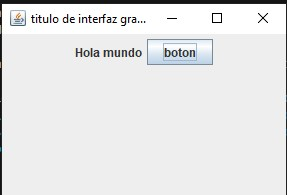
\includegraphics[width=0.4\textwidth,keepaspectratio]{img/img_primer_uno}
	\end{figure}
	\begin{figure}[H]
		\centering
		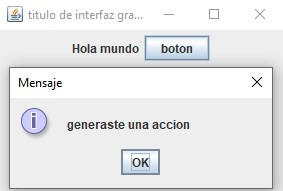
\includegraphics[width=0.4\textwidth,keepaspectratio]{img/img_primer_dos}
	\end{figure}
\begin{itemize}		
		\item A continuacion el primer codigo que use para crear una ventana agregando demas componentes .
		\item Primero unas importaciones generales.
		\item Luego instanciacion y creacion de los demas componentes.
		\item Se agrega los componentes al panel.
		\item Tambien se prioriza el tamaño.
	\end{itemize}
	\lstinputlisting[language=Java, caption={codigo1.java},numbers=left,]{src/codigo1.java}
	
	\clearpage
	

	
	
\begin{itemize}
		\item Este es una parte de los codigos que use, no obstante el codigo que genera neatbeans es un poco extenso y no modificable.
		\item Pero me ayudo a aprender como movia los contenedores y sus objetos .
		\item Apartir de esto podre usar y cortar los codigos cuando los genere yo mismo
		\item Al principio tuve dificultades con layout pero una vez haciendo diferentes codigos y visualizarlos cada uno entendi como funcionaba.
\end{itemize}
	\begin{lstlisting}[language=Java,caption={Analizando codigo generado por NeatBeans},numbers=left,][H]
package pruebas_interfaz;


import javax.swing.*;
import java.awt.*;
import java.awt.event.ActionEvent;
import java.awt.event.ActionListener;




public class Menu1 extends JFrame {

    private JPanel  menu;
    private JButton jugar;
    private JButton juego_Perzonalizado;
    private JButton salir;

    public Menu1() {
        p.setSize(800, 500);
        initComponents();
        this.setLocationRelativeTo(null);
        this.setTitle("Menu");
        this.setVisible(true);
    }

    private void initComponents() {

        menu  = new JPanel();
        jugar = new JButton();
        juego_Perzonalizado = new JButton();
        salir = new JButton();
        menu.setBackground(new Color(0,0,0));

        jugar.setText("Jugar");
        jugar.addActionListener(new ActionListener() {
            public void actionPerformed(ActionEvent evt) {
                Juego a = new Juego();
                cambiarPanel(a);
            }
        });

        juego_Perzonalizado.setText("Juego Perzonalizado");
        juego_Perzonalizado.addActionListener(new ActionListener() {
            public void actionPerformed(ActionEvent evt) {
                JuegoPersonalizado JP = new JuegoPersonalizado();
                cambiarPanel(JP);
            }
        });

        salir.setText("Exit");
        salir.addActionListener(new ActionListener() {
            public void actionPerformed(ActionEvent evt) {
                System.exit(0);
            }
        });

        GroupLayout MenuLayout = new GroupLayout(menu);
        menu.setLayout(MenuLayout);

        MenuLayout.setHorizontalGroup(
            MenuLayout.createParallelGroup(GroupLayout.Alignment.LEADING)
            .addGroup(MenuLayout.createSequentialGroup()
                .addGap(109, 109, 109)
                .addComponent(jugar, GroupLayout.PREFERRED_SIZE, 200, GroupLayout.PREFERRED_SIZE)
                .addGap(0, 0, 800))
            .addGroup(GroupLayout.Alignment.TRAILING, MenuLayout.createSequentialGroup()
                .addContainerGap(GroupLayout.DEFAULT_SIZE, 800)
                .addComponent(salir, GroupLayout.PREFERRED_SIZE, 200, GroupLayout.PREFERRED_SIZE)
                .addGap(71, 71, 71))
            .addGroup(MenuLayout.createSequentialGroup()
                .addGap(298, 298, 298)
                .addComponent(juego_Perzonalizado, GroupLayout.PREFERRED_SIZE, 200, GroupLayout.PREFERRED_SIZE)
                .addContainerGap(302, 800))
        );
        MenuLayout.setVerticalGroup(
            MenuLayout.createParallelGroup(GroupLayout.Alignment.LEADING)
            .addGroup(MenuLayout.createSequentialGroup()
                .addGap(132, 132, 132)
                .addComponent(jugar, GroupLayout.PREFERRED_SIZE, 45, GroupLayout.PREFERRED_SIZE)
                .addGap(60, 60, 60)
                .addComponent(juego_Perzonalizado, GroupLayout.PREFERRED_SIZE, 45, GroupLayout.PREFERRED_SIZE)
                .addPreferredGap(LayoutStyle.ComponentPlacement.RELATED, 100, 800)
                .addComponent(salir, GroupLayout.PREFERRED_SIZE, 45, GroupLayout.PREFERRED_SIZE)
                .addGap(73, 73, 73))
        );

        GroupLayout layout = new GroupLayout(getContentPane());
        getContentPane().setLayout(layout);
        layout.setHorizontalGroup(
            layout.createParallelGroup(GroupLayout.Alignment.LEADING)
            .addComponent(menu, GroupLayout.DEFAULT_SIZE, GroupLayout.DEFAULT_SIZE, 800)
        );
        layout.setVerticalGroup(
            layout.createParallelGroup(GroupLayout.Alignment.LEADING)
            .addComponent(menu, GroupLayout.DEFAULT_SIZE, GroupLayout.DEFAULT_SIZE, 800)
        );

        menu.getAccessibleContext().setAccessibleName("");

        pack();
    }


    private void cambiarPanel(JPanel p){
        p.setSize(800, 500);
        p.setLocation(0,0);
        menu.removeAll();
        menu.add(p);
        menu.revalidate();
        menu.repaint();
    }
}


\end{lstlisting}
\begin{itemize}
		
			\item En este fragmento de codigo Java,he creado una interfaz grafica de un tablero utilizando Java Swing y AWT. La interfaz incluye una cuadricula de 100 botones dispuestos en un panel (jPanel1) y botones de direccion (arriba, abajo, izquierda, derecha) en otro panel (jPanel2).
		\item La creacion que me reduce el codigo es con un array. Cada boton se identifica con un nombre unico utilizando la formula setName((i%10) + "" + ((99-i)/10)).
		\item Se implementaron manejadores de eventos para los botones de direccion, registrando la direccion seleccionada (arriba, abajo, izquierda, derecha) al ser clickeados.
		\item Al hacer clic en cualquier boton en el area principal (jPanel1), se ejecuta el metodo botonActionPerformed, actualizando las coordenadas x e y del juego segun la posicion del boton clickeado.
		\item Las ubicaciones de los componentes en la interfaz se logra mediante el uso de GroupLayout, simplificando la estructura y organizacion del codigo.
		\item Demostrando que puedo crear y ubicar objetos en un interfaz grafica
\end{itemize}
	\begin{lstlisting}[language=Java,caption={Creando la interfaz de tablero},numbers=left,][H]

package pruebas_interfaz;
import javax.swing.*;
import java.awt.*;
import java.awt.event.ActionEvent;
import java.awt.event.ActionListener;

public class Juego extends javax.swing.JPanel {
    private JButton[] boton = new JButton[100];
    private JButton jugar = new JButton();
    private JButton arriba = new JButton();
    private JButton abajo = new JButton();
    private JButton derecha = new JButton();
    private JButton izquierda = new JButton();
    private int x, y, direccion;
    private JPanel jPanel1;
    private JPanel jPanel2;

    public Juego() {
        initComponents();
    }
    private void initComponents() {

        jPanel1 = new JPanel(new GridLayout(10, 10));
        boton = new JButton[100];
        for (int i = 0; i < 100; i++) {
            boton[i] = new JButton();
            boton[i].setName((i%10) + "" + ((99-i)/10));
            jPanel1.add(boton[i]);
            boton[i].setBorder(BorderFactory.createEtchedBorder());
            boton[i].addActionListener(new ActionListener() {
                public void actionPerformed(ActionEvent e) {
                    botonActionPerformed(e);
                }

            });
        }
        jPanel2 = new JPanel(new GridLayout(2,2));
        jugar = new JButton();
        arriba = new JButton();
        abajo = new JButton();
        derecha = new JButton();
        izquierda = new JButton();

        arriba.setText("ar");
        arriba.addActionListener(new ActionListener() {
            public void actionPerformed(ActionEvent evt) {
                direccion = 2;
                System.out.println(2);
            }
        });

        izquierda.setText("iz");
        izquierda.addActionListener(new ActionListener() {
            public void actionPerformed(ActionEvent evt) {
                direccion = 1;
                System.out.println(1);
            }
        });

        derecha.setText("de");
        derecha.addActionListener(new ActionListener() {
            public void actionPerformed(ActionEvent evt) {
                direccion = 4;
                System.out.println(4);
            }
        });

        abajo.setText("ab");
        abajo.addActionListener(new ActionListener() {
            public void actionPerformed(ActionEvent evt) {
                direccion = 3;
                System.out.println(3);
            }
        });


        GroupLayout layout = new GroupLayout(this);
        this.setLayout(layout);
        layout.setHorizontalGroup(layout.createParallelGroup(GroupLayout.Alignment.LEADING)
                .addGroup(layout.createSequentialGroup()
                .addComponent(jPanel1, GroupLayout.PREFERRED_SIZE, 500, GroupLayout.PREFERRED_SIZE)                .addPreferredGap(javax.swing.LayoutStyle.ComponentPlacement.RELATED, 77, Short.MAX_VALUE)
                .addGroup(layout.createParallelGroup(javax.swing.GroupLayout.Alignment.TRAILING)
                    .addGroup(layout.createSequentialGroup()
                        .addComponent(izquierda, javax.swing.GroupLayout.PREFERRED_SIZE, 50, javax.swing.GroupLayout.PREFERRED_SIZE)
                        .addGap(56, 56, 56))
                    .addComponent(arriba, javax.swing.GroupLayout.PREFERRED_SIZE, 50, javax.swing.GroupLayout.PREFERRED_SIZE)
                    .addComponent(abajo, javax.swing.GroupLayout.PREFERRED_SIZE, 50, javax.swing.GroupLayout.PREFERRED_SIZE))
                .addPreferredGap(javax.swing.LayoutStyle.ComponentPlacement.RELATED)
                .addComponent(derecha, javax.swing.GroupLayout.PREFERRED_SIZE, 50, javax.swing.GroupLayout.PREFERRED_SIZE)
                .addGap(61, 61, 61)));
        layout.setVerticalGroup(  layout.createParallelGroup(GroupLayout.Alignment.LEADING)
                .addComponent(jPanel1, GroupLayout.DEFAULT_SIZE, 500, Short.MAX_VALUE)
                .addGroup(layout.createSequentialGroup()
                .addGap(132, 132, 132)
                .addComponent(arriba, javax.swing.GroupLayout.PREFERRED_SIZE, 50, javax.swing.GroupLayout.PREFERRED_SIZE)
                .addPreferredGap(javax.swing.LayoutStyle.ComponentPlacement.RELATED)
                .addGroup(layout.createParallelGroup(javax.swing.GroupLayout.Alignment.BASELINE)
                    .addComponent(derecha, javax.swing.GroupLayout.PREFERRED_SIZE, 50, javax.swing.GroupLayout.PREFERRED_SIZE)
                    .addComponent(izquierda, javax.swing.GroupLayout.PREFERRED_SIZE, 50, javax.swing.GroupLayout.PREFERRED_SIZE))
                .addPreferredGap(javax.swing.LayoutStyle.ComponentPlacement.RELATED)
                .addComponent(abajo, javax.swing.GroupLayout.PREFERRED_SIZE, 50, javax.swing.GroupLayout.PREFERRED_SIZE)
                .addGap(0, 206, Short.MAX_VALUE)));
    }

    private void botonActionPerformed(ActionEvent e) {
        int num = Integer.parseInt(((JButton)e.getSource()).getName());
        this.x = (num/10) +1;
        this.y = (num%10) +1;
    }


    public void casilla(){
        
    }
}
\end{lstlisting}
	
		\begin{itemize}
			\item Hasta este punto estuve modificando las variables y reordenandolo para que pueda ser un poco mas facil de comprender aunque aun me falta.
			\item Primero en posicion de elementos:
			\item Utilice principalmente 3 cosas para agregar juntar y posicionar
			\item Primero para agregar cosas es ".addComponent" ingresando 4 el componente y el tamaño
			\item Segundo para agrupar los componentes de forma paralela ".addGroup(layout.createSequentialGroup()"
			\item Y ultimo para poder posicionar es ".addGap" ingresando 3 numeros min, "distancia adecuada" y la distancia era la que yo ingresaba
			\item Todo esto con 2 metodos .setHorizontal(layout.createParallelGroup(  ...   y .setVertical(layout.createParallelGroup( ...   que era para ubicarlo de manera horizontal y vertical
			\item .addGap lo posiciona desde arriba a la izquierda hasta abajo a la derecha en esas direcciones
		\end{itemize}	
	\lstinputlisting[language=Java, caption={codigo1.java},numbers=left,]{src/codigo2.java}
	
	\begin{figure}[H]
		\centering
		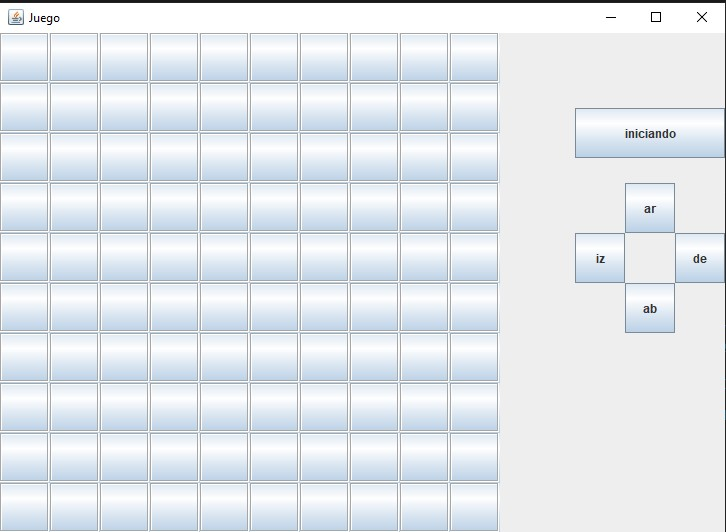
\includegraphics[width=0.8\textwidth,keepaspectratio]{img/img_tercero.jpg}
	\end{figure}

			
		\begin{itemize}
			\item En el siguiente codigo se puede ver que se agrego colores a los botones ademas de funcionalidades para empezar el juego
			\item El uso de setBackground(color ..) para los botones o para jpanel.
			\item Uso de action listener para conectar los botones con el videojuego
			\item Se coloco solo un boton para re pintar los botones y para actualizar la lista del ejercito con sus posiciones
			
		\end{itemize}
		\begin{lstlisting}[language=Java,caption={Creando la interfaz de tablero},numbers=left,][H]

import javax.swing.*;
import java.awt.*;
import java.awt.event.ActionEvent;
import java.awt.event.ActionListener;
import java.lang.reflect.Array;
import java.util.ArrayList;

public class Juego extends JPanel {
    private JButton[] boton = new JButton[100];
    private boolean turno;
    private JButton arriba;
    private JButton abajo;
    private JButton derecha;
    private JButton izquierda;
    private int x, y, direccion, x_x, y_y;
    private JPanel jPanel1;
    private JButton iniciarTurno;
    private Reinos reinos;

    public Juego() {
        initComponents();
        reinos = new Reinos();
        reinos.Reinos();
        this.turno = true;
        System.out.println(reinos.toString());
    }


    private void initComponents() {
        Color colora = new Color(0, 56, 43);
        Color colorb = new Color(25, 65, 47);
        jPanel1 = new JPanel(new GridLayout(10, 10));
        int lado = 500;
        boton = new JButton[100];
        for (int i = 0; i < 100; i++) {
            boton[i] = new JButton();
            if((i%2==0 && i/10%2 == 0) || (i/10%2==1 && i%2==1 )){
                boton[i].setBackground(colora);
            }else{
                boton[i].setBackground(colorb);
            }
            boton[i].setName((i%10) + "" + ((99-i)/10));
            jPanel1.add(boton[i]);
            boton[i].setBorder(BorderFactory.createEtchedBorder());
            boton[i].addActionListener(new ActionListener() {
                public void actionPerformed(ActionEvent e) {
                    botonActionPerformed(e);
                }
                
            });
        }
        int ladoBoton = 50;
        iniciarTurno = new JButton();
        arriba = new JButton();
        abajo = new JButton();
        derecha = new JButton();
        izquierda = new JButton();

        arriba.setBackground(new Color(200,50,50));
        arriba.setText("ar");
        arriba.addActionListener(new ActionListener() {
            public void actionPerformed(ActionEvent evt) {
                direccion = 2;
                System.out.println(2);
            }
        });

        izquierda.setBackground(new Color(50,200,50));
        izquierda.setText("iz");
        izquierda.addActionListener(new ActionListener() {
            public void actionPerformed(ActionEvent evt) {
                direccion = 1;
                System.out.println(1);
            }
        });

        derecha.setBackground(new Color(50,50,200));
        derecha.setText("de");
        derecha.addActionListener(new ActionListener() {
            public void actionPerformed(ActionEvent evt) {
                direccion = 4;
                System.out.println(4);
            }
        });

        abajo.setBackground(new Color(200,250,100));
        abajo.setText("ab");
        abajo.addActionListener(new ActionListener() {
            public void actionPerformed(ActionEvent evt) {
                direccion = 3;
                System.out.println(3);
            }
        });
        iniciarTurno.setText("iniciando");
        iniciarTurno.addActionListener(new ActionListener() {
            public void actionPerformed(ActionEvent evt) {
                moviendoReino(evt);
                repaint();
            }
        });

        GroupLayout layout = new GroupLayout(this);
        this.setLayout(layout);
        layout.setHorizontalGroup(layout.createParallelGroup(GroupLayout.Alignment.LEADING)
                .addComponent(jPanel1, lado, lado, lado)
                .addGroup(layout.createSequentialGroup()
                    .addGap(lado+65,lado+65,lado+65)
                    .addComponent(izquierda, ladoBoton, ladoBoton, ladoBoton)
                    .addGap(5, 5, 5)
                    .addGroup(layout.createParallelGroup(GroupLayout.Alignment.TRAILING)
                        .addComponent(arriba, ladoBoton, ladoBoton, ladoBoton)
                        .addComponent(abajo , ladoBoton, ladoBoton, ladoBoton)) 
                    .addGap(5, 5, 5)
                    .addComponent(derecha, ladoBoton, ladoBoton, ladoBoton))
                .addGroup(layout.createSequentialGroup()
                    .addGap(lado, lado +75, lado+ 75)
                    .addComponent(iniciarTurno, ladoBoton, ladoBoton + 100, ladoBoton+100)
                )
        );
        layout.setVerticalGroup(layout.createParallelGroup(GroupLayout.Alignment.LEADING)
                .addComponent(jPanel1, lado, lado, lado)
                .addGroup(layout.createSequentialGroup()
                    .addGap(150, 150, 150)
                    .addComponent(arriba, ladoBoton, ladoBoton, ladoBoton)
                    .addGap(5, 5, 5)
                    .addGroup(layout.createParallelGroup(GroupLayout.Alignment.TRAILING)
                        .addComponent(derecha, ladoBoton, ladoBoton, ladoBoton)
                        .addComponent(izquierda, ladoBoton, ladoBoton, ladoBoton))
                    .addGap(5, 5, 5)
                    .addComponent(abajo, ladoBoton, ladoBoton, ladoBoton))
                .addGroup(layout.createSequentialGroup()
                    .addGap(400,400,400)
                    .addComponent(iniciarTurno, ladoBoton, ladoBoton, ladoBoton)      
                )
        );
    }


    //acciones y funciones de los botones
    private void botonActionPerformed(ActionEvent e) {
        int num = Integer.parseInt(((JButton)e.getSource()).getName());
        this.x = (num/10) +1;
        this.y = (num%10) +1;
    }
    private void moviendoReino(ActionEvent e) {
        if(reinos.verificarPosicionLibreEjercitos(x , y)){//veridficar si la casilla que presiono tiene un ejercito
            System.out.println("-----" + reinos.verificarPosicionLibreEjercitos(x, y));
            x_x = x;
            y_y = y;
            movimientoCopia();
            if(reinos.verificarPosicionLibreEjercitos(x_x, y_y)){
                System.out.println("estuvo libre la siguiente posicion");
                movimiento();
            }else if(reinos.verificarAmigoPosicion(x_x, y_y, reinos.getReinos().get(reinos.buscarEjercito(x_x,y_y)))){
                System.out.println("Hay un amigo en la siguiente posicion");
            }else{
                System.out.println("Enemigo a la vista");
                movimiento();
            }
            System.out.println(reinos.toString());

            if(true)
                turno = false;
                
            if(reinos.verificarReinos())
                System.exit(0);
        }
    }
    private void movimiento(){
        switch (direccion) {
            case 1: this.x--;  break;//izquierda
            case 2: this.y++;  break;//arriba
            case 3: this.y--;  break;//abajo
            case 4: this.x++;  break;//derecha
            default:System.out.println("Error: movimiento() --> Juego");  break;
        }
    }
    private void movimientoCopia(){
        switch (direccion) {
            case 1: x_x--;  break;//izquierda
            case 2: y_y++;  break;//arriba
            case 3: y_y--;  break;//abajo
            case 4: x_x++;  break;//derecha
            default:System.out.println("Error: movimiento() --> Juego-otro");  break;
        }
    }
}
\end{lstlisting}
		\begin{itemize}
			\item Ejecucion del main y visualizacion de ventana de juego
		\end{itemize}	
	
	\begin{figure}[H]
		\centering
		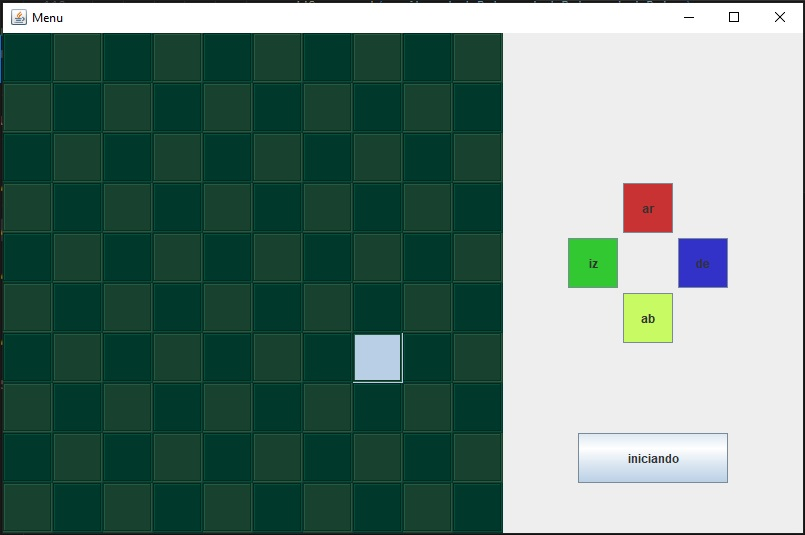
\includegraphics[width=0.8\textwidth,keepaspectratio]{img/ventana_de_juego.jpg}
	\end{figure}

		\begin{itemize}
			\item Desde el menu direccionar al panel del juego
		\end{itemize}
	\begin{figure}[H]
		\centering
		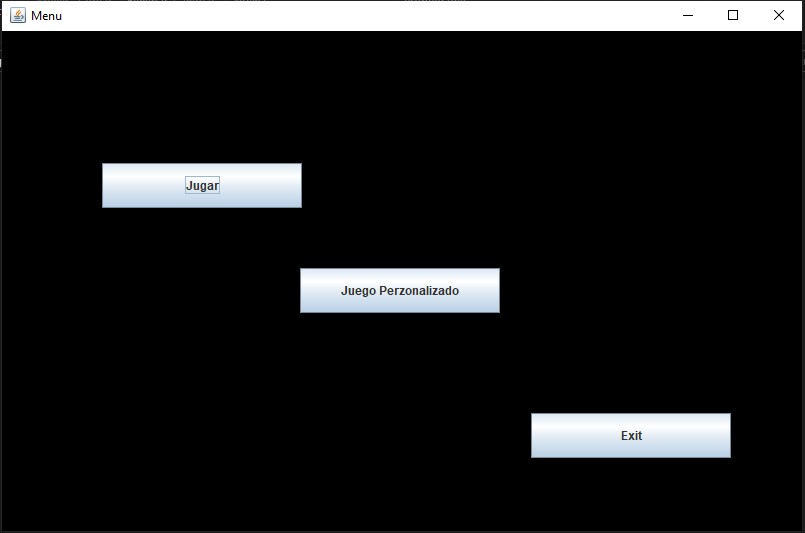
\includegraphics[width=0.8\textwidth,keepaspectratio]{img/ventana_menu.jpg}
	\end{figure}

	\subsection{Estructura de laboratorio 22}
	\begin{itemize}	
		\item El contenido que se entrega en este laboratorio es el siguiente:
	\end{itemize}
	
\begin{lstlisting}[style=ascii-tree]
lab_22
|---Arquero.java
|---Caballero.java
|---Ejercito.java
|---Espadachin.java
|---Juego.java
|---Lancero.java
|---Latex
| |---Nueva carpeta
| |---programacion_lab22__jquispemad_v1.0.log
| |---programacion_lab22__jquispemad_v1.0.pdf
| |---programacion_lab22__jquispemad_v1.0.synctex.gz
| |---programacion_lab22__jquispemad_v1.0.tex
| |---src
| | |---codigo1.java
| | |---img_primer_dos.jpg
| | |---img_primer_uno.jpg
| | |---insercion.png
| | |---logo_abet.png
| | |---logo_episunsa.png
| | |---logo_unsa.jpg
| | |---ventana_de_juego.jpg
| | |---ventana_menu.jpg
|---Main.java
|---Mapa.java
|---Menu.java
|---pruebas_interfaz
| |---JuegoPersonalizado.java
| |---PanelFondo.java
| |---pruebas.java
|---Reinos.java
|---Soldado.java
|---Tablero.java

\end{lstlisting}    


	\section{\textcolor{red}{Rúbricas}}
	
	\subsection{\textcolor{red}{Entregable Informe}}
	\begin{table}[H]
		\caption{Tipo de Informe}
		\setlength{\tabcolsep}{0.5em} % for the horizontal padding
		{\renewcommand{\arraystretch}{1.5}% for the vertical padding
		\begin{tabular}{|p{3cm}|p{12cm}|}
			\hline
			\multicolumn{2}{|c|}{\textbf{\textcolor{red}{Informe}}}  \\
			\hline 
			\textbf{\textcolor{red}{Latex}} & \textcolor{blue}{El informe está en formato PDF desde Latex,  con un formato limpio (buena presentación) y facil de leer.}   \\ 
			\hline 
			
			
		\end{tabular}
	}
	\end{table}
	
	
	\subsection{\textcolor{red}{Rúbrica para el contenido del Informe y demostración}}
	\begin{itemize}			
		\item El alumno debe marcar o dejar en blanco en celdas de la columna \textbf{Checklist} si cumplio con el ítem correspondiente.
		\item Si un alumno supera la fecha de entrega,  su calificación será sobre la nota mínima aprobada, siempre y cuando cumpla con todos lo items.
		\item El alumno debe autocalificarse en la columna \textbf{Estudiante} de acuerdo a la siguiente tabla:
	
		\begin{table}[ht]
			\caption{Niveles de desempeño}
			\begin{center}
			\begin{tabular}{ccccc}
    			\hline
    			 & \multicolumn{4}{c}{Nivel}\\
    			\cline{1-5}
    			\textbf{Puntos} & Insatisfactorio 25\%& En Proceso 50\% & Satisfactorio 75\% & Sobresaliente 100\%\\
    			\textbf{2.0}&0.5&1.0&1.5&2.0\\
    			\textbf{4.0}&1.0&2.0&3.0&4.0\\
    		\hline
			\end{tabular}
		\end{center}
	\end{table}	
	
	\end{itemize}
	
	\begin{table}[H]
		\caption{Rúbrica para contenido del Informe y demostración}
		\setlength{\tabcolsep}{0.5em} % for the horizontal padding
		{\renewcommand{\arraystretch}{1.5}% for the vertical padding
		%\begin{center}
		\begin{tabular}{|p{2.7cm}|p{7cm}|x{1.3cm}|p{1.2cm}|p{1.5cm}|p{1.1cm}|}
			\hline
    		\multicolumn{2}{|c|}{Contenido y demostración} & Puntos & Checklist & Estudiante & Profesor\\
			\hline
			\textbf{1. GitHub} & Hay enlace URL activo del directorio para el  laboratorio hacia su repositorio GitHub con código fuente terminado y fácil de revisar. &2 &X &2 & \\ 
			\hline
			\textbf{2. Commits} &  Hay capturas de pantalla de los commits más importantes con sus explicaciones detalladas. (El profesor puede preguntar para refrendar calificación). &4 &X &4 & \\ 
			\hline 
			\textbf{3. Código fuente} &  Hay porciones de código fuente importantes con numeración y explicaciones detalladas de sus funciones. &2 &X &1.5 & \\ 
			\hline 
			\textbf{4. Ejecución} & Se incluyen ejecuciones/pruebas del código fuente  explicadas gradualmente. &2 &X &2 & \\ 
			\hline			
			\textbf{5. Pregunta} & Se responde con completitud a la pregunta formulada en la tarea.  (El profesor puede preguntar para refrendar calificación).  &2 &X &2 & \\ 
			\hline	
			\textbf{6. Fechas} & Las fechas de modificación del código fuente estan dentro de los plazos de fecha de entrega establecidos. &2 &X &2 & \\ 
			\hline 
			\textbf{7. Ortografía} & El documento no muestra errores ortográficos. &2 &X &2 & \\ 
			\hline 
			\textbf{8. Madurez} & El Informe muestra de manera general una evolución de la madurez del código fuente,  explicaciones puntuales pero precisas y un acabado impecable.   (El profesor puede preguntar para refrendar calificación).  &4 &X &2 & \\ 
			\hline
			\multicolumn{2}{|c|}{\textbf{Total}} &20 & &17.5 & \\ 
			\hline
		\end{tabular}
		%\end{center}
		%\label{tab:multicol}
		}
	\end{table}
	
\clearpage

\section{Referencias}
\begin{itemize}			
	\item \url{https://www.w3schools.com/java/default.asp}
	\item \url{https://www.geeksforgeeks.org/insertion-sort/}
\end{itemize}	
	
%\clearpage
%\bibliographystyle{apalike}
%\bibliographystyle{IEEEtranN}
%\bibliography{bibliography}
			
\end{document}